% \begin{frame}{Git no decide nada}
%     \begin{block}{DISCLAIMER - Mundos paralelos}
%         Nos vamos a encontrar con varias situaciones donde git tiene que resolver que hacer frente a dos versiones "recientes" de un algo (archivo, repo, etc). Por ejemplo, repo local vs repo remoto, archivo commiteado vs archivo pusheado (por otra persona). Esto es complicado!
%     \end{block}
%
%     \pause
%
%     En la clase anterior, mencionamos que git es muy sencillo y no toma decisiones por nosotros. Vamos a ver un ejemplo claro de esto.
%
% \end{frame}

\begin{frame}[t]{Mandando fruta}

    \begin{ejercicio}{Ejercicio de a 2 personas en máquinas: \emoji{grapes} y \emoji{pear}}
        \begin{enumerate}\begin{small}
            \pause
        \item \emoji{grapes} y \emoji{pear}: vamos a seguir usando el repo anterior (el de \emoji{christmas-tree} y \emoji{jack-o-lantern}), asegurense de pullear lo ultimo asi seguimos desde ahí.
            \pause
            \item \emoji{grapes}:
            crear un archivo \textit{ensalada.txt} con una linea que diga "bowl". aca va a ir la ensalada. commitear y pushear.
            \item \emoji{pear}: pullear para obtener el archivo \textit{ensalada.txt} con solo "bowl".
            \pause
            \item \emoji{grapes} y \emoji{pear}: hagan \textit{commits} (1 cada) agregando algunos nombres de frutas a su ensalada en la misma linea que "bowl".
            \pause
            \item \emoji{grapes}: hacer \textit{git push} con sus cambios.
            \pause
            \item \emoji{pear}: bajarse los cambios del repositorio remoto con \textit{git pull}. Resolver el conflicto (!) y pushear
            \pause
            \item \emoji{grapes}: bajarse los nuevos cambios.
            \pause
        \item \emoji{grapes} y \emoji{pear}: repetir estos pasos con los roles invertidos si aun no lo hicieron (en un nuevo archivo).
        \end{small}\end{enumerate}
    \end{ejercicio}

\end{frame}

\begin{frame}[t]{Muy importante (?)}
    \begin{figure}[ht]
        \begin{center}
            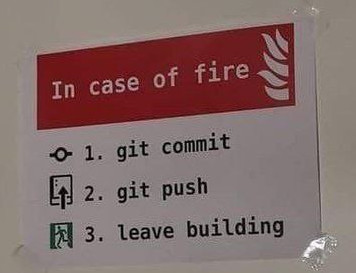
\includegraphics[height=2.6in]{images/in-case-of-fire.jpg}
        \end{center}
    \end{figure}
\end{frame}
